\documentclass{article}
\setlength{\parskip}{5pt} % esp. entre parrafos
\setlength{\parindent}{0pt} % esp. al inicio de un parrafo
\usepackage{amsmath} % mates
\usepackage[sort&compress,numbers]{natbib} % referencias
\usepackage{url} % que las URLs se vean lindos
\usepackage[top=15mm,left=20mm,right=20mm,bottom=25mm]{geometry} % margenes
\usepackage{hyperref} % ligas de URLs
\usepackage{graphicx} % poner figuras
\usepackage[spanish]{babel} % otros idiomas

\author{Claudia Lizeth Hern\'andez Ram\'irez} % author
\title{Homework 1 - Movimiento Browniano} % titulo
\date{\today}

\begin{document} % inicia contenido

\maketitle % cabecera



% RESUMEEEEEEEEEEEEEEEN
\begin{abstract} % resumen
  \centering
  LA distancia es directamente proporcional a los par\'ametros n800, n8000n, n80000 (largo de caminata) y a dimensi\'on.
\end{abstract}


% INTRODUCCIOOOOOOOOOOOON
\section{Introducci\'{o}n}\label{intro} % seccion y etiqueta

Este trabajo tiene como objetivo analizar y comprender el efecto que provoca modificar los par\'ametros de la dimensi\'on y el largo de caminata sobre la distancia que recorre una part\'icula. Movimiento Browniano. 




% DESARROLLOOOOOOOOOOOO
\section{Desarrollo}\label{desarrollo} % Desarrollo de la tarea

Comenc\'e por determinar el recorrido de mi part\'icula modicando en el programa (figura 1) \citep{DraElisa} los par\'ametros \texttt{DIM} y \texttt{DUR} que representan las dimensiones (3, 6, 9, 27, 81 y 243) y el largo que durar\'a la caminata (800, 8000 y 80000 pasos) respectivamente; estos datos los capturé en un archivo de excel (figura 2) \cite{excel}.
Para comenzar a graficar se utiliz\'o la librer\'ia \texttt{ggplot2}. \citep{ejemplo} \cite{ggplot}
Se import\'o el archivo de excel antes creado \texttt{DATAHW1} y con \texttt{geom-boxplot} \citep{geom}  gener\'e las primeras cajas para n=80000;sin embargo Rstudio acomoda las cajas en un orden que no era entendible (figura 3) \cite{primerintento} . Con \texttt{fct-relevel} \citep{fct} logr\'e ordenar de forma manual el eje X para que pudiera ser entendible(figura 4).
Para lograr que n80000, n8000 y n800 \citep{superponer} \cite{rggvideo} estuvieran en un mismo gr\'afico utilice el s\'imbolo de suma (+) posterior a este s\'imbolo coloqué de nuevo un \texttt{geom-boxplot} pero con eje X de n8000, posterior mente otro \texttt{geom-boxplot} con eje de n800 (figura 5).
Con la librer\'ia \texttt{scales} añad\'i el t\'itulo principal de la gr\'afica, el subt\'itulo y los nombre de los ejes \texttt{X} y \texttt{Y}.
Finalmente este es el c\'odigo (figura 6) con el cu\'al pude obtener la gr\'afica (figura 7) que describ\'ia el comportamiento del eje  \texttt{distancia} con la variaci\'on de los par\'ametros antes mencionados.


%CONCLUSIOOOON
\section{Conclusi\'on}

La distancia que se recorre conforme se aumenta de dimensiones se muestra en un comportamiento ascendente, este patr\'on se replica para n= 800, n=8000 y n=80000, es decir, la distancia es directamente proporcional al n\'umero de dimensiones.
De igual forma, si analizamos una sola dimensi\'on, por ejemplo D27, es evidente que la distancia mayor recorrida es mayor conforme aumentamos el largo de caminata.

Al momento de trabajar.
Tuve un par de dificultades para realizar esta tarea, al inicio pretend\'ia colocar todos los datos obtenidos de la caminata en forma de vector en Rstudio, sin embargo no logr\'e acomodar la gr\'afica de manera correcta, en la figura 8 se puede observar como se graficaba.
Posteriormente en la librer\'ia ggplot v\'i que era mucho mas sencillo trabajar las gr\'aficas, pero segu\'ia teniendo el mismo problema de no saber como sobreponer las gr\'aficas as\'i que, se me ocurri\'o generar un boxplot para cada \texttt{n} y despu\'es juntarlas ya que hab\'ia visto que se pod\'ia juntar una gr\'afica boxplot con una de puntos y pens\'e que se pod\'ia hacer lo mismo con dos gr\'aficos similares, lo intent\'e y funcion\'o, el resto fue cuesti\'on solamente de dar formato.
Personalmente creo que la escala logar\'itmica del eje Y no est\'a del todo clara ya que las boxplot de la D81 y D243 no se logran visualizar abiertamente, de ahi en fuera estoy contenta con mi trabajo ya que personalmente esta materia se me complica.




%COMIENZAN LAS FIGURAS E IMAGENES
\begin{figure} % figura
    \centering
    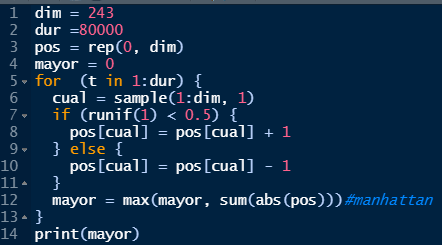
\includegraphics[width=150mm]{figura 1.PNG} % archivo
    \caption{Programa utilizado para determinar la distancia recorrrida. }
    \label{figura 1}
\end{figure}

\begin{figure} % figura
    \centering
    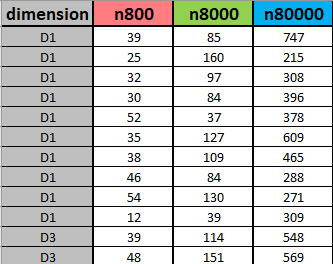
\includegraphics[width=100mm]{figura 2.PNG} % archivo
    \caption{Fragmento de datos capturados de caminata en excel - DATAHW1}
    \label{figura 2}
\end{figure}

\begin{figure} % figura
    \centering
    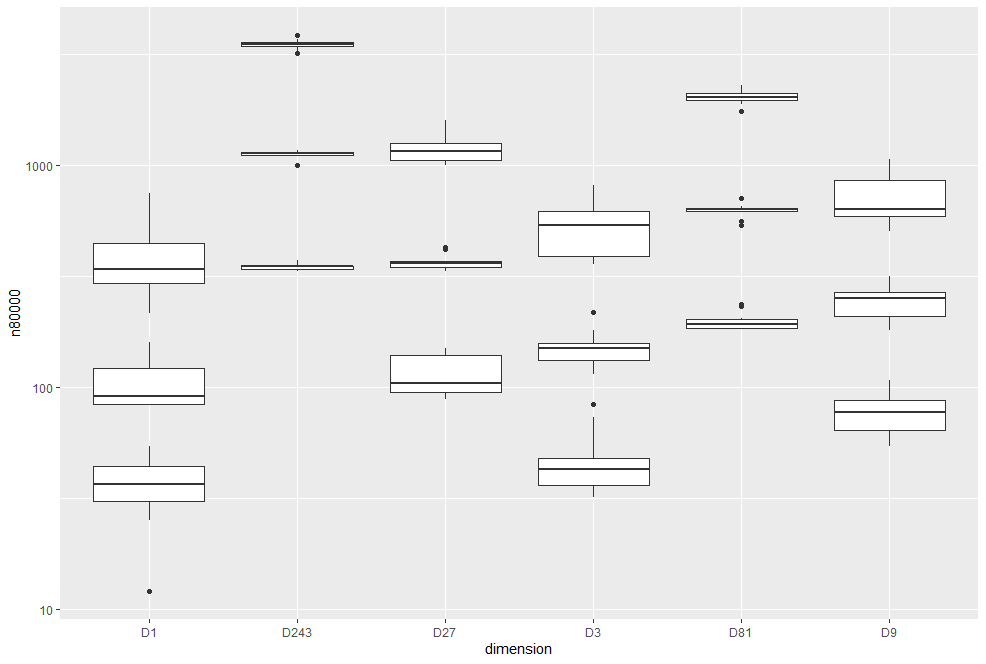
\includegraphics[width=150mm]{figura 3.PNG} % archivo
    \caption{Primer intento de gr\'afica, eje X desordenado.}
    \label{figura 3}
\end{figure}

\begin{figure} % figura
    \centering
    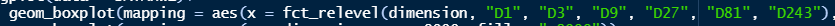
\includegraphics[width=150mm]{figura 4.PNG} % archivo
    \caption{Implementaci\'on de fct-relevel para reordenar manualmente eje X.}
    \label{figura 4}
\end{figure}

\begin{figure} % figura
    \centering
    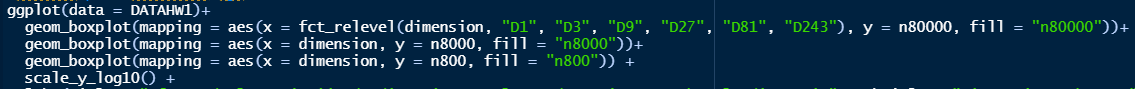
\includegraphics[width=100mm]{figura 5.PNG} % archivo
    \caption{geom-boxplot + geom-boxplot + geom-boxplot.}
    \label{figura 5}
\end{figure}

\begin{figure} % figura
    \centering
    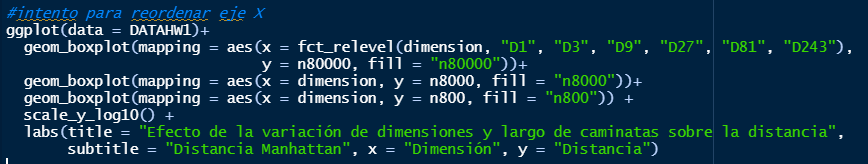
\includegraphics[width=100mm]{figura 6.PNG} % archivo
    \caption{c\'odigo final para generar BOXPLOT final.}
    \label{figura 6}
\end{figure}

\begin{figure} % figura
    \centering
    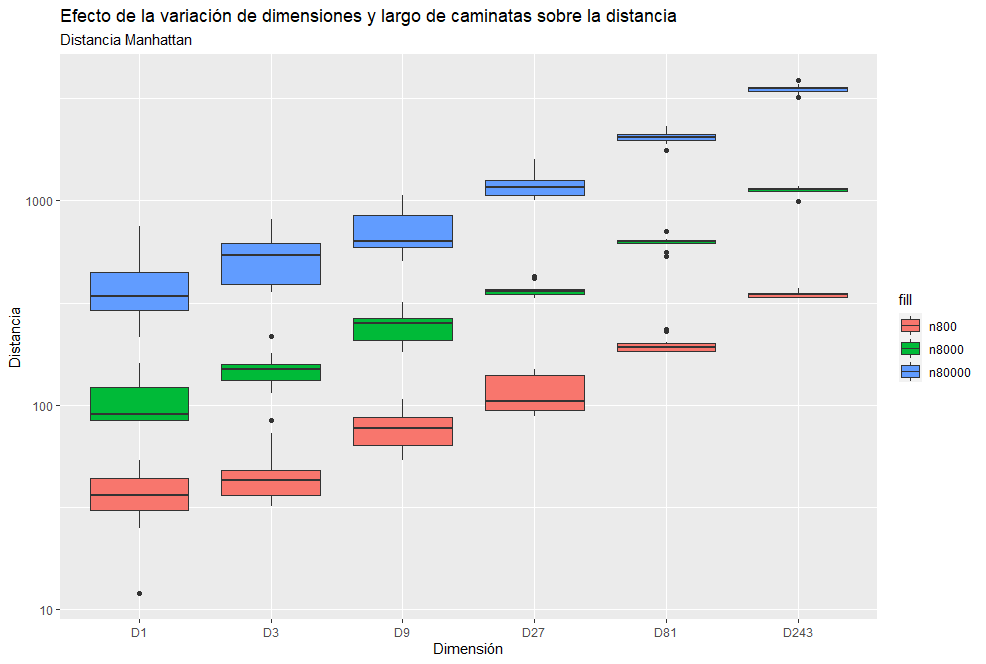
\includegraphics[width=160mm]{figura 7.PNG} % archivo
    \caption{BOXPLOT final.}
    \label{figura 7}
\end{figure}

\begin{figure} % figura
    \centering
    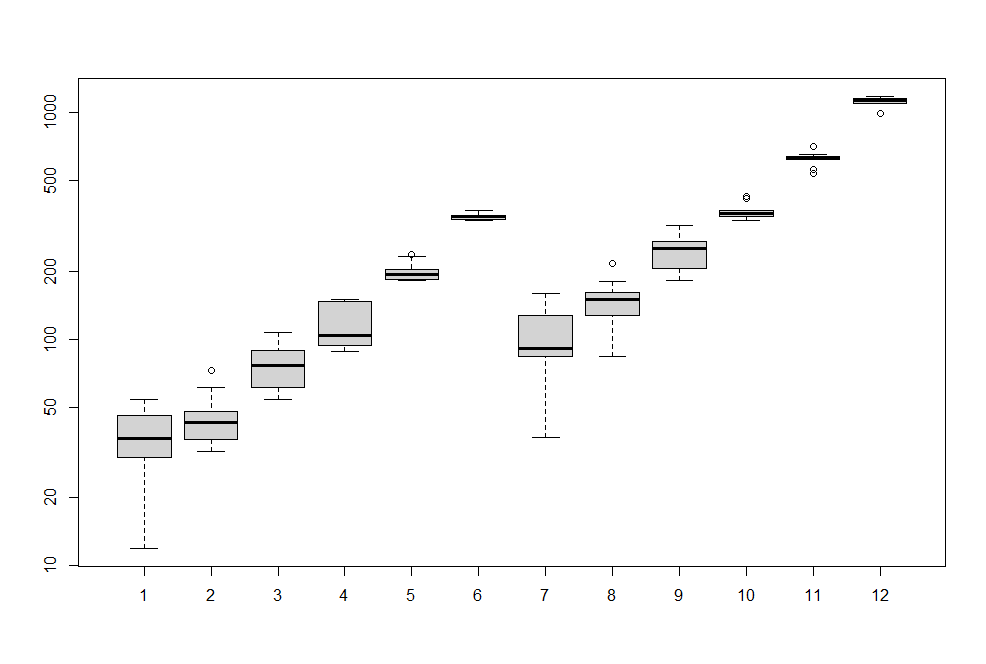
\includegraphics[width=150mm]{figura 8.PNG} % archivo
    \caption{Primer intento de boxplot.}
    \label{figura 8}
\end{figure}

% BIBLIOGRAFIAAAAAAS
\bibliography{referencias}
\bibliographystyle{plainnat}
\end{document}
